\documentclass[12pt,oneline,a4paper,numbib]{ouparticle}
\usepackage{array,multirow,graphicx}
\usepackage{pdflscape}% for landscape

\begin{document}

\title{MSE and dynamic state variable model with sigma function}

\author{%
\name{Nekane Alzorriz}
\address{European Commission, Joint Research Centre (JRC), Sustainable Resources Directorate, Water and Marine Resources Unit, Via Enrico Fermi 2749, 21027 Ispra, Italy.}
\email{nekane.alzorriz@gmail.com}
\and
\name{Jan Jaap Poos}
\address{Wageningen Marine Research, PO Box 68, 1970 AB IJmuiden, The Netherlands.}
\email{janjaap.poos@wur.nl}}

\abstract{
TBD

Use DSVM with a tuning parameter that measures how important is to be near optimal.

We use this DSVM to investigate how fishing locations change in response when fish biology is incorporated.}

\date{\today}

\keywords{word1; word2; word3; and word4}

\maketitle


\section{Introduction}
\label{sec1}

The new Common Fisheries Policy marks a number of key changes to European fisheries management, including the introduction of multi-annual management plans aimed at achieving the Maximum Sustainable Yield (MSY) for all stocks and the gradual introduction of a landings obligation (LO) to encourage more selective fishing practices. Their implementation cannot be seen in isolation from each other as strategies aimed at one objective may have consequences for achieving the other. LO and catch quotas should provide incentives for change in the fisheries, including adoption through taking up selective gears and spatiotemporal effort allocation.

Fisheries management typically focuses on the sustainable exploitation of single target species, but the potentially negative effects on, for example, reaching other species conservation objectives, should also be evaluated. Achieving single species MSY in complex and dynamic fisheries targeting multiple species (mixed fisheries) is challenging because achieving the objective for one species may mean missing the objective for another \cite{Ulrich2017}. There is no unique way of translating the single-species MSY objective to the multispecies case. Maximisation of yield from one stock will generally require different strategies than maximisation of yield from another.  Whatever the management regime, the performance of management strategies is conditioned by population dynamics, but also by exploitation dynamics, and particularly by the response of the fleets to management measures. Management strategy evaluation (MSE; \cite{Sainsbury2000, Smith1994, Venables2009}) seeks to study the likely implications of potential harvest policies, or strategies, on the operation of a mixed fishery and on the fished stocks. 

MSE involves building a simulation model for the entire process under study, complex enough both to address the current knowledge and uncertainty on the dynamics of fish stocks under fishing pressure, the effect on fishers of variations in stock status and availability, and their responses to those changes and those in management regimes \cite{Venables2009}. At the same time being simple enough to build and calibrate reliably with the available data. More comprehensive MSEs may also take the effects of the fishery on the broader environment, and economic and social effects into account \cite{Dichmont2008, Fulton2007}. 

There is a substantial literature addressing the question of effort allocation in fisheries and the more general question of state-dependent foraging decisions in ecological systems \cite{ClarkandMangel2000,Houston1999}. New tools for state-dependent behaviour of individual fishing vessels, translated into behaviour of the fleet and implemented using stochastic dynamic programming \cite{Alzorriz2017,Batsleer2015, Dowling2011, Poos2010} have been developed. These models generally predict the effect in the short term (within a year) by optimizing an objective function and determine which area best suits this behaviour given the set of incentives that exist (which may also depend on factors such as size, home port, distance to fishing grounds and expected catch rates). Effects of e.g. relocation costs of marine protected areas, the implementation of the landings obligation, have been modelled under these approaches. In contrast, to enable longer term prediction accounting for the impact of these choices on the populations and consequently on the future yields, this fleet dynamic model should be coupled to a biological dynamic model where the feedback between fleet and stock dynamics are explicity modelled.
 
A key module in any fisheries MSE, and our primary concern here, is the fleet-dynamics model combined with a biological dynamic model, i.e. if the fleet dynamic model results in a short term movement of vessels to allocate effort both spatially and temporally, we also expect longer term changes to occur in fish populations and the economy of the fishery \cite{Alzorriz2017}. Such combination needs to be responsive to all the drivers that influence and motivate the actual fleet and to respect existing constraints \cite{Venables2009}. The drivers will include the (real or perceived) local abundance and catchability of the fished stocks and various resource costs, principally that of fuel. The constraints will include the obvious management-imposed constraints such as levels of total allowable catch, and economical constraints such as the contribution of the annual fines for exceeding catch quotas.

Using a MSE, the main objective of this work is to understand the fleet dynamics in a spatially and temporally heterogeneous mixed quota-regulated fishery when reducing from unmanaged (unconstrained catch quota) to MSY managed and to compare it with a situation where discards are allowed in order to assess on the biological and economic consequences. If LO and catch quotas are not fully enforced, there will be an incentive to continue discarding. Therefore, this manuscript tends to understand the likely adaptive change in fishing patterns that will help us to understand if this leads to a better balance between quotas and catches.

%Since maximizing effort does not maximize catch, the question is if there is an optimum fishing rate that would lead to a maximum yield.


\section{Methods}
\label{sec2}

\subsection{Stock structure and dynamics}
\label{sec2.1}

For purposes of model simplicity, we consider a hypothetical mixed fishery on two species. The fishery is modelled in a individual based dynamic state variable model. In order to allow for fishing effort allocation, the model is seasonally and spatially explicit. The dynamics of the two fish species are governed by a simple age-structured model that is also seasonally and spatially explicit. In the age structured model for the fish species, individuals are assumed to be born at age 0, and in season 1. The number of fish of age $a$ at year $y$, in season $s$ and area $p$ is written as $N (a, y, s, p)$. The number of new-born individuals in the model is independent of the size of the adult population. Individuals can be born in each of the areas, such that  
\begin{equation*}
N (0, y, 1, p) = R (p)
\end{equation*}

Mortality in the model can occur from catches in the fishery, and natural causes such as predation, diseases, and scenesens. However, for simplicity we assume that his natural mortality is negligible. Althought such absence of natural mortality impossible in reality, one could argue that the model thus mimics long-lived species. The decrease in population numbers is thus the result of the catches ($C (a, y, s, p)$), which are in turn a function of age dependent catchability $q(a)$, and fishing effort $E (y,s,p)$ in any time, season, and area. 

\begin{equation*}
C (a, y, s, p) = q(a) * E(y,s,p)
\end{equation*}

and 
\begin{equation*}
N (a, y, s, p) = N (a, y, s, p) - C (a, y, s, p) 
\end{equation*}

Migration for each species is defined by a matrix that defines the migration to ($top$) and from ($fromp$) each of the areas in the model. Its dimensions are thus equal to the number of areas in the model.  The migration in population numbers ($Mig (a, 1, s, top, fromp)$) is thus the proportion ($p (a, y, s, i, fromq, top)$) of the population available or vulnerable to fishing after migration occurs.   
\begin{equation*}
Mig (a, 1, s, top, fromp) = Mig(a, 1, s, top, fromp) + N (a, y, s, fromp) * p (a, y, s, i, fromq, top)
\end{equation*}

and then population numbers
\begin{equation*}
N (a, y, s, top) = N (a, y, s, top) +  Mig (a, 1, s, top, fromp)
\end{equation*}

Life history traits inputted are: (i)  during the first season, specie 1 spawns in ``A'', while specie 2 spawns in ``B'', (ii) every season, 20\% of specie 1 and 2 migrate from area ``A'' to ``B'' and from ``B'' to ``A'', (iii) growth following the von Berttalanffy equation (with the following parameters: $L\infty= 20$, $k= 0.093$), (iv) age-weight relationship ($W= L\infty*(1-e^{-k*a})$), (v) at the beginning of each year the fishing recruitment is stablish in 100.

The purpose of the operating model is not to reproduce the entire complexity of a real mixed fishery, but to define plausible hypothesis about population dynamics and then to implement the processes of interest, i.e., changes in population abundance, to finally measure the effect of the potential consequences associated with the fishers optimal choice location underlying assumption of the current state-dependat behaviour of individual fishing vessels.

\subsection{The dynamic-state variable model}
\label{sec2.2}

We develop models for state-dependent behaviour of individual fishing vessels, translated into behaviour of the fleet and implemented using stochastic dynamic programming \cite{Alzorriz2017, Batsleer2015, ClarkandMangel2000, Dowling2011, Houston1999, Poos2010}. 

In order to calculate the optimal state dependent choices during the year, we start by defining the contribution of the annual fines for exceeding landings or catches quotas at the end of the year to the utility is: 
\begin{equation*}
\Phi (C_i, Q_i^C, F_i^C) = -\sum_{i} (max(0, (C_i - Q_i^C)\times F_i^C),
\end{equation*}

where $C_i$ are the cumulative annual catches, for species i. $Q_i^C$ are the annual quota for catches. $F_i^C$ are the fines per unit weight for exceeding catch quota. Hence, starting with $V (C, Q, F, t) = \Phi (C, Q, F)$ we assigned a probability to each region patch proportional to its profit associated at that point in the season (t), given the quota remaining. Following \cite{Dowling2011}, if $V^\ast$ is the profit at the optimal location for a given Q and t, we set
\begin{equation*}
\Delta (Q_i^C, t) = V^\ast (C_i, Q_i^C, F_i^C, t) - V (C_i, Q_i^C, F_i^C, t),
\end{equation*}

and then define the probability of fishing particular area as
\begin{equation*}
P (Q_i^C, t) = \frac{e^-\Delta (Q_i^C, t)/\sigma} {\sum_{i}(e^-\Delta (Q_i^C, t)/\sigma)},
\end{equation*}

where $\sigma$ is a tuning parameter that measures how important is to be near optimal.  A high value of sigma would mean that probabilities are uniform and vessels are distributed uniformly along the different fishing areas, while a low sigma value would mean that vessels concentrate in the optimal location. For computations, we use $\sigma = 40$, to introduce some error in the decision making (Table \ref{t:fishery}).

Then, we can iterate backwards in time and fine the optimal choice in terms of location and discarding behaviour for all possible states, combinig the net revenue obtained from the sale of fish and costs of a fishing trip and the effect of the annual fines when exceeding anuual quota. Prices of fish have been assumed to be constant over fish age and time. The variable costs include fuel costs ($\sim{40\%}$), crew share ($\sim{35\%}$) and gear mantainance ($\sim{4\%}$)). Fuel costs depend on gear used, trip effort and fuel price. Fuel costs were set to 150 \texteuro day\textsuperscript{-1}. Gear maintenance costs were assumed proportional to fishing effort, landing costs proportional to the total weight landed, and crew share variable costs proportional to the income from catches (Table~\ref{t:fishery}).


\begin{table}[!h]
\centering
\caption{Fishery parameterization.}
\label{t:fishery}
\resizebox{\textwidth}{!}{%
\begin{tabular}{@{}|lc|lc|lc|@{}} 
\hline
\textbf{model}                              &               & \textbf{Variable costs}                        &      &\textbf{Market value}&  \\ \hline
& & & & & \\
number of vessels                           &700            &fuel costs (Euro day\textsuperscript{-1})       & 150  & sp1 (Euro kg\textsuperscript{-1})                 & 1000 \\ 
$\sigma $                                   & 40            &gear maintenance (Euro day\textsuperscript{-1}) & 287  & sp2 (Euro kg\textsuperscript{-1})                 & 1000   \\
number of areas                             & 2             &crew share                                      & 35\% & & \\
number of seasons                           & 6             &landing costs (Euro t\textsuperscript{-1})      & 0    & &\\
intial quota $Q_sp1$ and $Q_sp2$            & 200           &                                                &      & & \\
& & & & & \\\hline
\end{tabular}
}
%\hline
%\textbf{model}                              &   \\ \hline
%\\
%number of vessels                                 &700\\
%$\sigma $                                         & 40\\
%number of areas                                   & 2 \\
%number of seasons                                 & 6\\
%intial quota Q1 and Q2                            & 200\\
%\\\hline
%\textbf{Variable costs}                              &\\ \hline
%\\
%fuel costs (Euro day\textsuperscript{-1})       & 1240\\
%gear maintenance (Euro day\textsuperscript{-1}) & 287 \\
%crew share                                      & 35\%\\
%landing costs (Euro t\textsuperscript{-1})      & 121\\
%\\\hline
%\textbf{Market value (Euro kg\textsuperscript{-1})}&  \\ \hline
%\\
%sp1                  & 1000 \\
%sp2                  & 1000   \\
%\\\hline 
%\end{tabular}
%}
\end{table}


% Prices of fish have been assumed to be constant over fish age and time.

%We assume high sigma values  to introduce some error in the decision making. A high sigma value is settled to run the model, therefore, we are forcing the model to have uniform probabilities along the different fishing patches. However, with this approach, there is a model time where vessels concentrate in the different locations in the same manner. Therefore, if at that moment we introduce a low sigma value, we force the model to concentrate probabilities in the optimal location.

%If we run each scenario 100 times, we will be able to reproduce the confidence intervals. Providing reference points for management purposes and providing information on the contribution of a fixed number of individuals to the spawning component of the population (spawning stock per recruitment model).

\subsection{Endogenously determined quotas}
\label{sec2.3}

Quota is determined endogenously by simple and relatively linear reduction in catch if fishing mortality exceeds Fmsy. This requires that fishing mortality for each stock must not exceed Fmsy, which is a limit reference point. An Optimum Yield (OY) is determined based on a MSY that must prevent overfishing, and that can be reduced from the MSY limit to take into account social, economic and precautionary considerations.  Therefore, quota is determined by a set of harvest control rule parameters consisting of the exploitaion rate at MSY.
related to the OY, which must be risk averse. 

\begin{equation*}
 U_{T+1} = U_{MSY}, 
\end{equation*}
\begin{equation*}
 Q_{i, T+1}^{L} = (U_{T+1}\times B_{T+1}),
\end{equation*}

%Given the landing parameters associated

%hr<- catches.n/ (catches.n+ pop)
%landings.ratio <- landings.n/ cathces.n
%OY <- 
%hr_MSY <- OY[OY_landings==max(OY_landingslandings),]_hr

prel.quota <-  sum(sweep((hr1wanted[1]/mean(hr1[,yy,]))* hr1[,yy,]*landings.ratio1[,yy,]*apply(pop1[,yy+1,,],c(1,2), sum) ,1,wts,"*"))/SIMNUMBER
        tac.constrained <- c(quota1[,yy,,]*0.85, quota1[,yy,,]*1.15)
        quota1[,yy+1,,] <- max(min(prel.quota, tac.constrained[2]), tac.constrained[1])
        
        
From an economic perspective, a linear increase towards maximum TAC is the optimal strategy under plausible assumptions on market demand for fish and harvesting cost, as shown in Froese et al., 2010. The economic rationale is that, beyond Blim, the stock is within safe biological limits, and as it becomes more and more productive, it is able to supply the market to an increasing extent. 

A linear reduction in fishing mortality has been implemented in Australia (DAFF 2007) a nd is common in the USA. The differences between a linear decline in fishing mortality and a linear decline in TAC are small, see Figure A2 in Appendix S4.     

estimating the hr Fisheries are managed by a total allowable catch (TAC). A maximum TAC is set for each stock so that the respective target biomass is maintained
on average. This maximum TAC may be taken as long as biomass fluctuations remain above Bmsy. 

- No quota constrained

- Through a yield per recruit model, knowing growth, harvest rates and recruitment we can estimate how much to reduce the quota for achieving the MSY.  Since maximizing effort does not maximize catch, the question is if there is an optimum fishing rate that would lead to a maximum yield. The principal purpose of yield per recruit models is to get an idea of the effect of selection pattern and fishing mortality on the yield from a fixed number of individuals that enters the fishery.

Therefore if we have a harvest rate of 0.32, we will need to reduce the harvest in a 68\%. Reduce quota in next run in 68\%. From this reduction in quota and the subsequent reduction in IQ, this scenario will be evaluated allowing and not allowing the fleet to discard. 

\subsection{Scenarios analysed}
\label{sec2.4}

Simulations have been performed under three different scenarios. All compared to an unmanaged fishery, with unconstrained quota for both species.

\begin{table}[!h]
\centering
\caption{}
\label{scenarios}
\resizebox{\textwidth}{!}{%
\begin{tabular}{|c |c | c | c |}
\hline
 \textbf{Scenario I}            & \textbf{Scenario II}                & \textbf{Scenario III}               & \textbf{ScenarioIV}           \\ 
 \textbf{Fulll avoidance of discards} & \textbf{Landings selectivity} & \textbf{Catch selectivity}          & \textbf{LO not fully enforced} \\ \hline
 & &  &\\
 No discarding allowed          & Discarding allowed                  & Discarding allowed                  & Discarding ocurred but not perceived \\
 Manager perceives $C$          & Manager perceives $L$ and $D$       & Manager perceives $L$ and $D$       & Manager only perceives $L$ \\
 assuming that $C = L$          & assuming that $C = L + D$           & assuming that $C = L + D$           & assuming that $C = L$  \\
 YPR based in $F_C$             & YPR based in $F_L$                  & YPR based in $F_C$                  &  YPR based in $F_L$  \\
 assuming $L/C=1$               & assuming $L/C \neq 1$               & assuming $L/C \neq 1$               & assuming $L/C=1$\\
  & &  &\\\hline
\end{tabular}
}
\end{table}
 
% \parbox[c]{2mm}{\multirow{7}{*}{\rotatebox[origin=c]{90}{\textbf{Naive manager}}}} 
% & &  \\
 %& Discarding allowed & \\
% & Manager only perceives $L$ &\\
% & assuming that $C = L$  &\\
% & YPR based in $F_L$  & \\
% & assuming $L/C=1$    & No discarding allowed\\
% & & $C = L$ \\\cline{1-2}
%  \parbox[c]{2mm}{\multirow{7}{*}{\rotatebox[origin=c]{90}{\textbf{Smart manager}}}} 
% & &  Advice and quota\\
% & Discarding allowed & based on $C = L$\\
% & Manager perceives $L$ and $D$ & \\
% & assuming that $C = L + D$ &\\
% & YPR based in $F_C$  &\\
% & assuming $L/C \neq 1$ &\\
%  & &  \\\hline
% & \textbf{NO LO}              & \textbf     {LO}                                  \\ \hline


\begin{enumerate}

\item
\textbf{Scenario I: Fulll avoidance of discards}, this scenario contemplates the LO with landings selectivity only and fulll avoidance of discards.
%decrease the quota on both species to reach the Fmsy.
%Reduce the IQs in the same percentage as the change in HR to reach the equilibrium (MSY). 

\item
\textbf{Scenario II: Landings selectivity},  under this scenario the fishery is under landings selectivity, only landings contribute to yield. Fishing mortality accounts for all catches, regardless wether these catches are landed or discarded. 

\item
\textbf{Scenario III: Catch selectivity},  under this scenario the fishery is under a full catch selectivity, but all discards are landed and contribute to yield. Fishing mortality accounts for all catches, regardless wether these catches are landed or discarded. This results generally in higher $F_{MSY}$.
%decrease the quota on both species to reach the Fmsy.
%Reduce the IQs in the same percentage as the change in HR to reach the equilibrium (MSY). 

\item 
\textbf{Scenario IV: LO not fully enforced}, if LO is not fully enforced, therefore, there will be the incentive to continue discarding. However the manager could think that is fully enforced and assumed that only what is landed contribute to yield. This is the typicall situation of a choke species, where the management target such as $F_{MSY}$ cannot be easily achieved, because reductions in TACS do not necessarily translate into the expected reduction in fishing mortality. Rather, they may translate into increased discards if the fishery is mixed and continues fishing for other species beyond the exhaustion of the TAC of the species in question.
en vez de plantearlo como que no es LO, podria plantearse como que realmente esta bajo el LO, pero no hay compliance y el manager no lo sabe. Por tanto los hr se estiman como si el C fueran L...
%decrease the quota on sp 1 and unconstrained quota for species 2.
%CONSTRAINED fishery for sp1 and UNCONSTRAINED sp2 (FIXING QUOTA SP2 to 200). Only sp1 is forced to try to reach the Fmsy. However discarding is allowed for both species.

%same as scenario II but allowing to discard only species 2.

%\item
%Scenario IV, Same as scenario I but allowing to discard sp2.
\end{enumerate}


\section{Results}
\label{sec3}


\newpage
\begin{landscape}
Scenario I:
%----------------------------------------------------------------------------------------------------------------------------------------
\begin{figure}[!h]
\centering
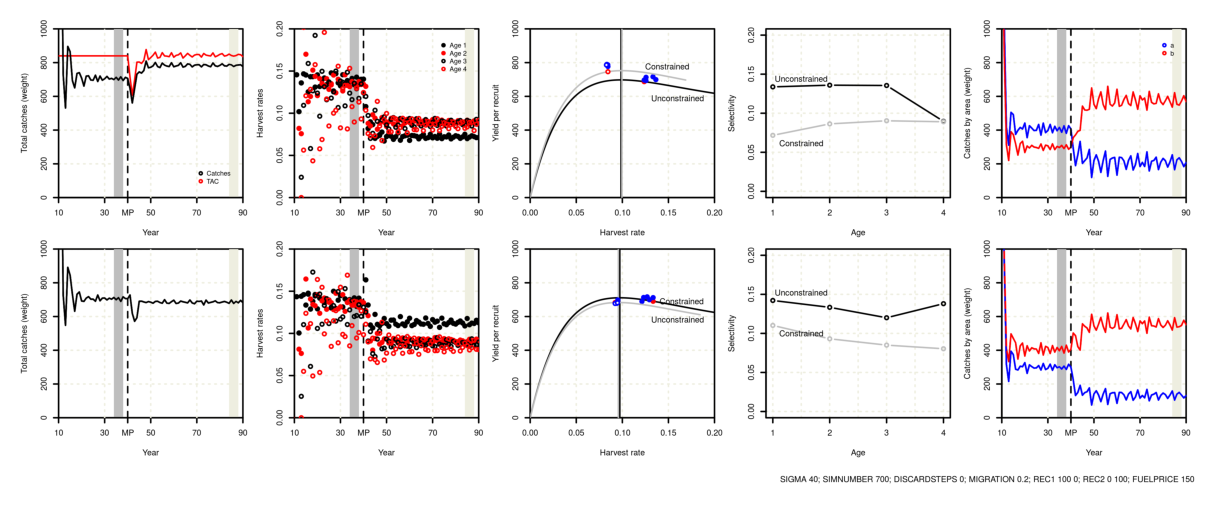
\includegraphics[width=\textheight,height=6cm]{Figures/Catch_LO.eps} 
\caption{}
\label{fig:catch_lo}
\end{figure}

\begin{figure}[!h]
\centering
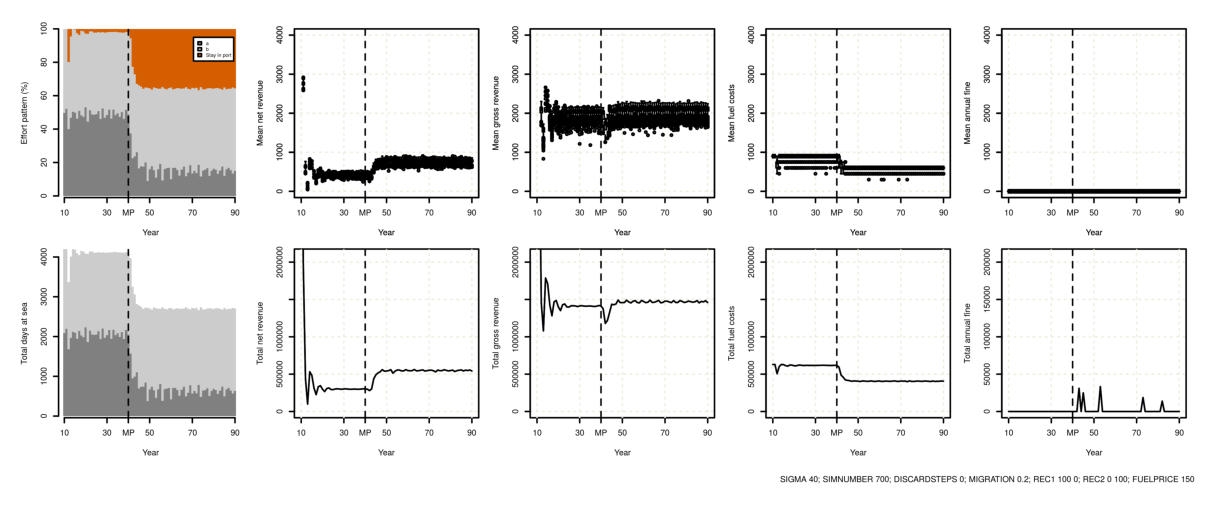
\includegraphics[width=\textheight,height=6cm]{Figures/Effort_LO.eps} 
\caption{}
\label{fig:effort_lo}
\end{figure}
\end{landscape}

%----------------------------------------------------------------------------------------------------------------------------------------
\newpage
\begin{landscape}
Scenario II:
%----------------------------------------------------------------------------------------------------------------------------------------
\begin{figure}[!h]
\centering
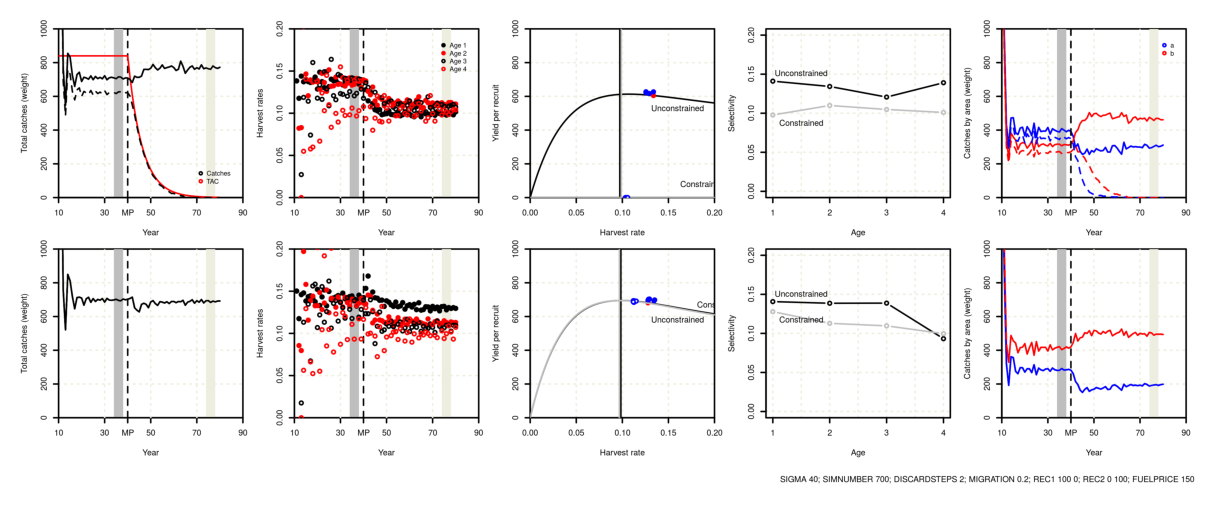
\includegraphics[width=\textheight,height=6cm]{Figures/Catch_LO_disc_YieldLand.eps} 
\caption{}
\label{fig:catch_lo}
\end{figure}

\begin{figure}[!h]
\centering
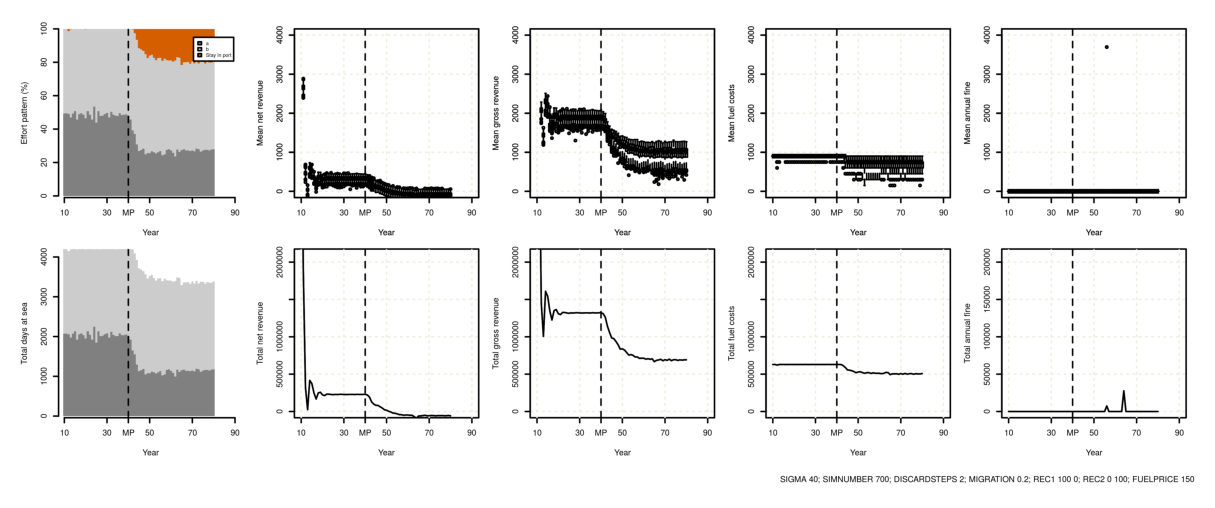
\includegraphics[width=\textheight,height=6cm]{Figures/Effort_LO_disc_YieldLand.eps} 
\caption{}
\label{fig:effort_lo}
\end{figure}
\end{landscape}

%----------------------------------------------------------------------------------------------------------------------------------------
\newpage
\begin{landscape}
Scenario III:
%----------------------------------------------------------------------------------------------------------------------------------------

\begin{figure}[!h]
\centering
\includegraphics[width=\textheight,height=6cm]{Figures/Catch_LO_smartmanager.eps} 
\caption{}
\label{fig:catch_lo}
\end{figure}

\begin{figure}[!h]
\centering
\includegraphics[width=\textheight,height=6cm]{Figures/Effort_LO_smartmanager.eps} 
\caption{}
\label{fig:effort_lo}
\end{figure}
\end{landscape}

%----------------------------------------------------------------------------------------------------------------------------------------
\newpage
\begin{landscape}
Scenario IV:
%----------------------------------------------------------------------------------------------------------------------------------------
\begin{figure}[!h]
\centering
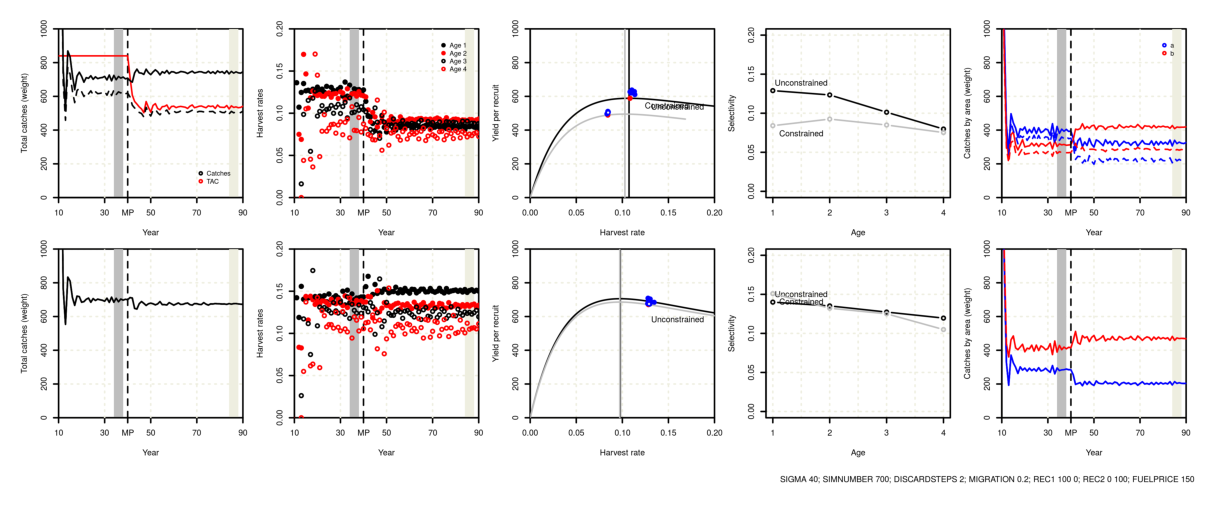
\includegraphics[width=\textheight,height=6cm]{Figures/Catch_LO_nocompliance.eps}  
\caption{}
\label{fig:catch_lo}
\end{figure}

\begin{figure}[!h]
\centering
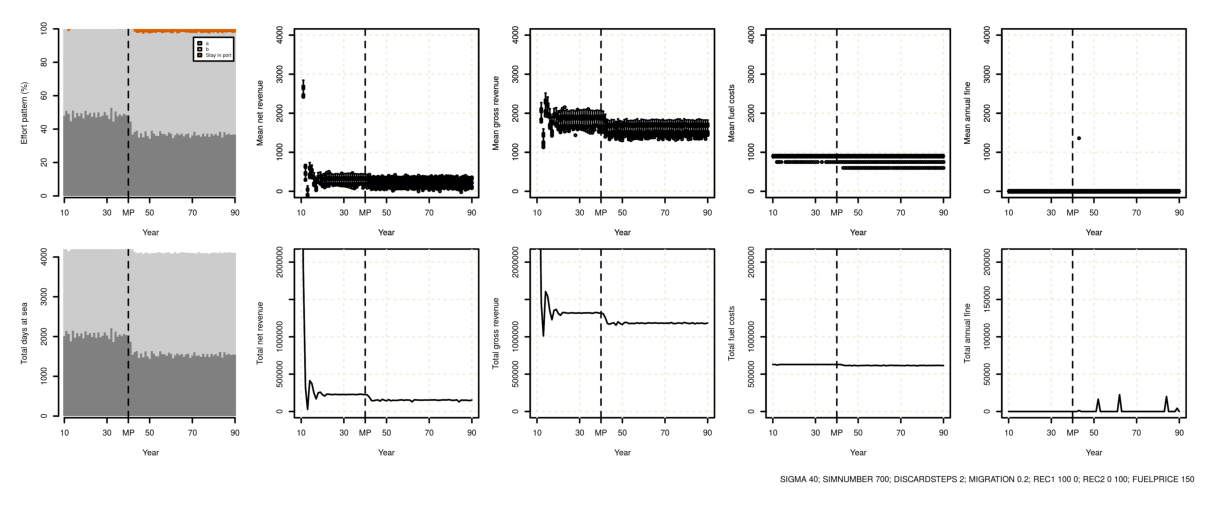
\includegraphics[width=\textheight,height=6cm]{Figures/Effort_LO_nocompliance.eps} 
\caption{}
\label{fig:effort_lo}
\end{figure}
\end{landscape}
%----------------------------------------------------------------------------------------------------------------------------------------

\subsection{Simulated catch decisions and location choice}
\label{sec3.1}

The largest yield (or catch) that can be taken from a species' stock over an indefinite period. Fundamental to the notion of sustainable harvest, the concept of MSY aims to maintain the population size at the point of maximum growth rate by harvesting the individuals that would normally be added to the population, allowing the population to continue to be productive indefinitely. Under the assumption of logistic growth, resource limitation does not constrain individuals’ reproductive rates when populations are small, but because there are few individuals, the overall yield is small. At intermediate population densities, also represented by half the carrying capacity, individuals are able to breed to their maximum rate. At this point, called the maximum sustainable yield, there is a surplus of individuals that can be harvested because growth of the population is at its maximum point due to the large number of reproducing individuals. Above this point, density dependent factors increasingly limit breeding until the population reaches carrying capacity. At this point, there are no surplus individuals to be harvested and yield drops to zero. The maximum sustainable yield is usually higher than the optimum sustainable yield and maximum economic yield

There is an extensive literature on fisheries economic theory in which the Gordon-Schaefer equilibrium production model is central (Gordon 1954, Schaefer 1957, Clark 1983). This theory holds that there is an economic TRP, the Maximum Economic Yield (MEY), which occurs at the effort level yielding the greatest margin of revenue over cost from the resource. 
For a linear cost curve, this inevitably occurs to the left of MSY on the fishing effort axis. Since Fmey occurs at lower levels of effort than Fmsy, the use of this economic Target Reference Point is less likely to result in biological overfishing than the use of Fmsy.

As a TRP, Fmey is responsive to any changes in the economic environment which affect either the value of fish, or the cost of fishing. It may also be dependent on changes in fish abundance, if market price increases with declining abundance and is independent of the availability of similar resources elsewhere. Subsidies or external economic considerations such as fuel taxes will also affect the location of an economic Reference Point (e.g. Panayotou 1988).

The effect of supply on fish prices may, under certain circumstances, result in higher total profit, or profit per unit catch, when total catch is reduced. This characteristic may be a consideration in setting target fishing levels or catches but is least likely to be effective in situations where fish prices are set by global markets, e.g. the tuna fishery for the canning industry.

The value of a unit weight of the landed catch may vary with the size of individual fish, and in multispecies fisheries with species composition. Both fish size and species composition are functions of fishing mortality, and based on purely economic criteria, may be used as target reference points. Even if the actual target F cannot be estimated, in theory, F could be adjusted in increments until the desirable target catch characteristics are achieved.

In considering TRPs based on economic criteria, it is important to be aware of the effect which the practice of discounting could have on reference points. In evaluating investment projects, including resource management, economists discount the future value of any commodity. Discount rates may be in the order of 10\%. In the case of a fishery where the population growth rate does not exceed the discount rate, then a strict application of economic theory would suggest that in the absence of other considerations (such as an economic value placed on recreational use of resources) the whole stock should be harvested now, and the proceeds of their sale invested. Long-lived species with slow growth rates, such as whales, clearly fall into this category. The blatant contradiction between this common economic approach, and the concept of sustainability, constitutes an unresolved paradox (Hilborn and Walters 1992).

\section{Discussion}
\label{sec4}
tbd
prellezo 2016, In the mid-term and without any consideration made in terms of the ecosystem functioning as a whole, the results obtained from applying any kind of exemption or flexibility are, simply, negative. Fishing beyond FMSY (even in one year) implies that there will be a penalty in the future. This penalty will come in the form of lower biomasses, that has the mixed effect of increasing the cost of fishing the same level of catches and reducing the total catch due to the lower abundances and the subsequent lower TACs.

\begin{notes}[Acknowledgements]
The content of this paper does not reflect the official opinion of the European Commission. Responsibility for the information and views expressed in this paper relies entirely with the authors.
\end{notes}

\newpage
\bibliographystyle{plain}
\bibliography{mylib}

\end{document}
